\documentclass[aspectratio=169]{beamer}

\usepackage[utf8]{inputenc}
\usepackage[T1]{fontenc}
\usepackage{graphicx}
\usepackage{listings}
\usepackage{xcolor}

\definecolor{codegreen}{rgb}{0,0.6,0}
\definecolor{codegray}{rgb}{0.5,0.5,0.5}
\definecolor{codepurple}{rgb}{0.58,0,0.82}
\definecolor{backcolour}{rgb}{0.95,0.95,0.92}

\lstdefinestyle{mystyle}{
    backgroundcolor=\color{backcolour},
    commentstyle=\color{codegreen},
    keywordstyle=\color{magenta},
    numberstyle=\tiny\color{codegray},
    stringstyle=\color{codepurple},
    basicstyle=\ttfamily\footnotesize,
    breakatwhitespace=false,
    breaklines=true,
    captionpos=b,
    keepspaces=true,
    numbers=left,
    numbersep=5pt,
    showspaces=false,
    showstringspaces=false,
    showtabs=false,
    tabsize=2
}

\lstset{style=mystyle}

\title{Statistical Data Analysis Project}
\author{Alexandre De Cuyper}
\date{February 22, 2024}
\institute{University of A Coruña}

\begin{document}

\frame{\titlepage}

\begin{frame}{Introduction}
    \begin{itemize}
        \item Analyze the powder X-ray diffraction data,
        \item Objectives and hypotheses: Investigating if there are significant differences in peak positions and intensity among crystals,
        \item Importance of the analysis: Understanding the change in structure of the crystals when changing the composition.
    \end{itemize}
\end{frame}

\begin{frame}{Data Overview}
    \begin{itemize}
        \item Overview of the dataset: Peaks from different crystals with compositions and varying 2 theta values.
        \item Key variables and their significance: `2_theta`, Composition, Intensity, and Cluster.
    \end{itemize}
\end{frame}

\begin{frame}[fragile]{Data Preprocessing}
    \begin{itemize}
        \item Cleaning and handling missing values.
        \item Transformation of data for analysis.
    \end{itemize}

    \begin{lstlisting}[language=R]
    > head(data)
      2_theta Ni75Co25 Ni50Co50 Ni25Co75   Co
    1    8.00     20.0    18.00    24.00 19.0
    2    8.05     19.5    21.98    23.01 20.5
    3    8.10     19.0    26.00    22.00 22.0
    4    8.15     19.0    27.49    21.50 25.0
    5    8.20     19.0    29.00    21.00 28.0
    6    8.25     17.0    24.53    24.98 24.5
    \end{lstlisting}
\end{frame}

\begin{frame}[fragile]{Exploratory Data Analysis}
    \begin{itemize}
        \item Visualizations and summary statistics.
        \item Identification of patterns and trends.
    \end{itemize}

    \begin{lstlisting}[language=R, basicstyle=\tiny\ttfamily]
    # Exploratory Data Analysis (EDA)
    ggplot(data, aes(x = `2_theta`)) +
  geom_ribbon(aes(ymin = 0, ymax = `Ni25Co75`, fill = "Ni25Co75"),
    alpha = 0.1, color = "green"
  ) +
  geom_ribbon(aes(ymin = 0, ymax = `Ni50Co50`, fill = "Ni50Co50"),
    alpha = 0.1, color = "red"
  ) +
  geom_ribbon(aes(ymin = 0, ymax = `Ni75Co25`, fill = "Ni75Co25"),
    alpha = 0.1, color = "blue"
  ) +
  geom_ribbon(aes(ymin = 0, ymax = `Co`, fill = "Co"),
    alpha = 0.1, color = "yellow"
  ) +
  labs(
    title = "Powder X-ray Diffraction of Ni_(1-x)Co_x perovskites",
    x = "2 theta",
    y = "Intensity",
    fill = "Composition"
  ) +
  scale_fill_manual(values = c(
    "Ni75Co25" = "blue", "Ni50Co50" = "red",
    "Ni25Co75" = "green", "Co" = "yellow"
  )) +
  theme_minimal()
    \end{lstlisting}
\end{frame}

\begin{frame}{Visualization of the Data}
    \begin{figure}
        \centering
        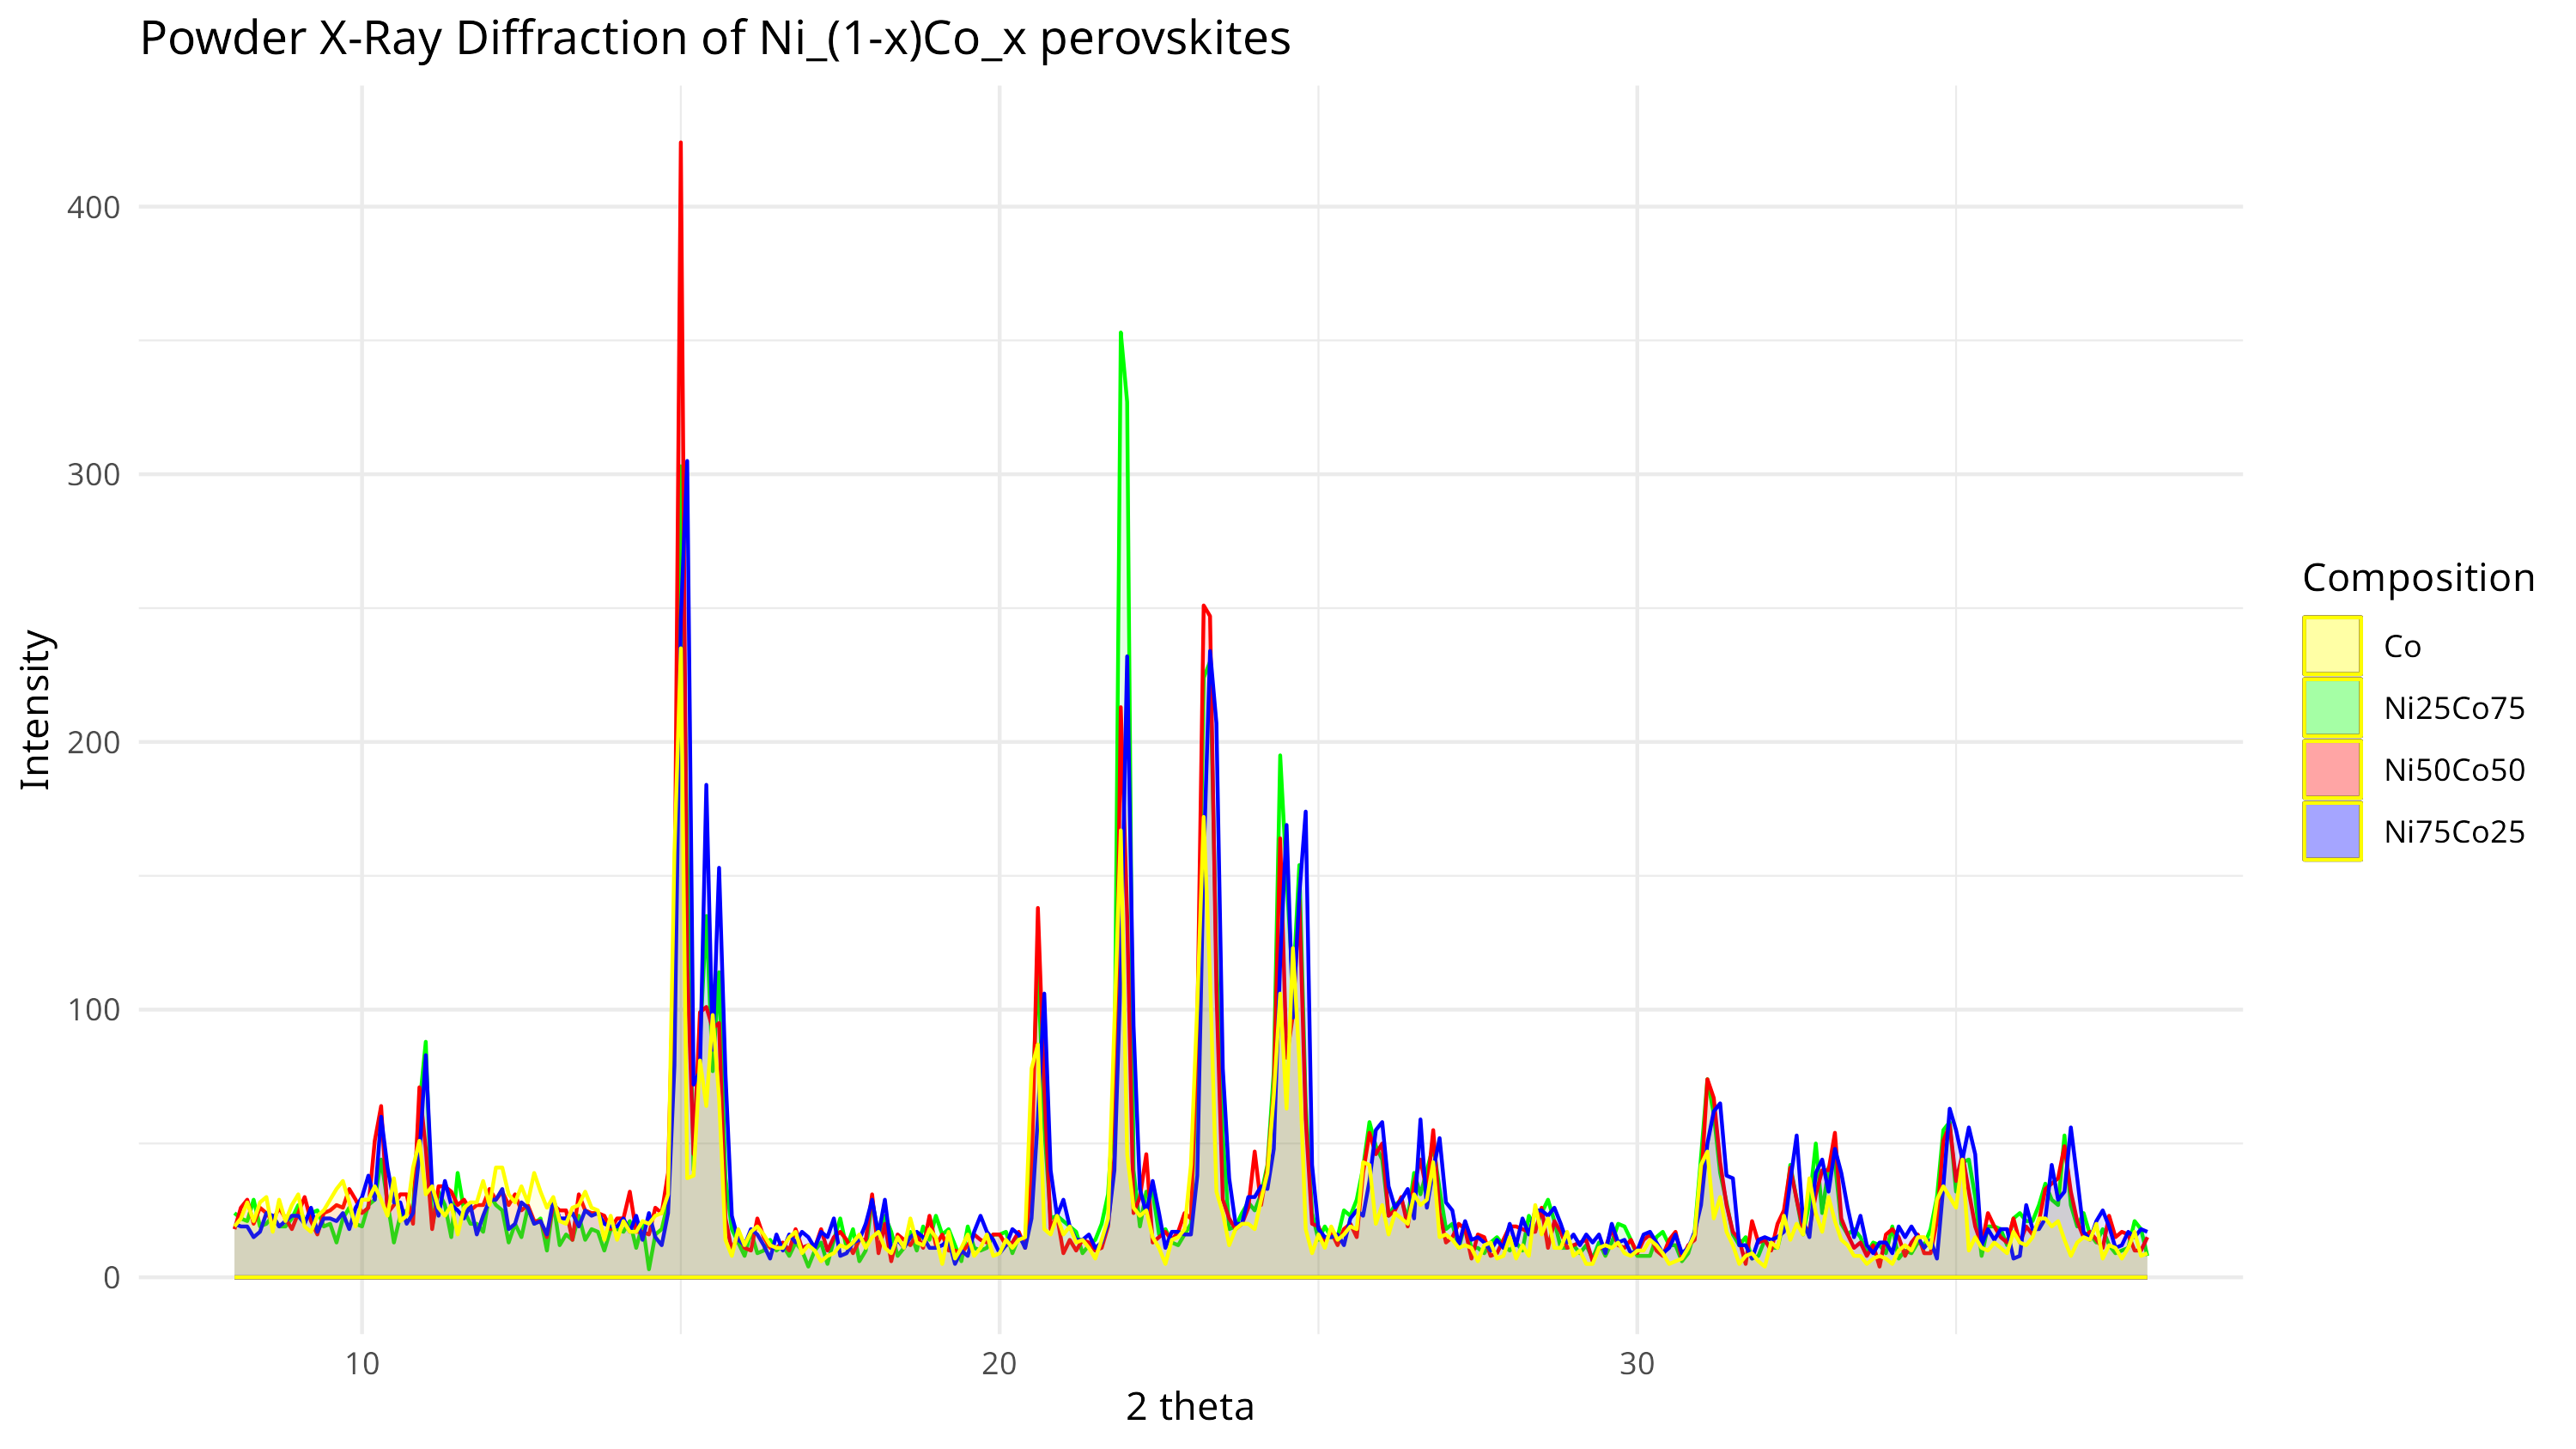
\includegraphics[width=1\textwidth]{../plot/graph_nb.png}
        \caption{Powder X-ray Diffraction of Ni\_(1-x)Co\_x perovskites}
        \label{fig:xrd}
    \end{figure}
\end{frame}

\begin{frame}{Visualization of the Data}
    \begin{figure}
        \centering
        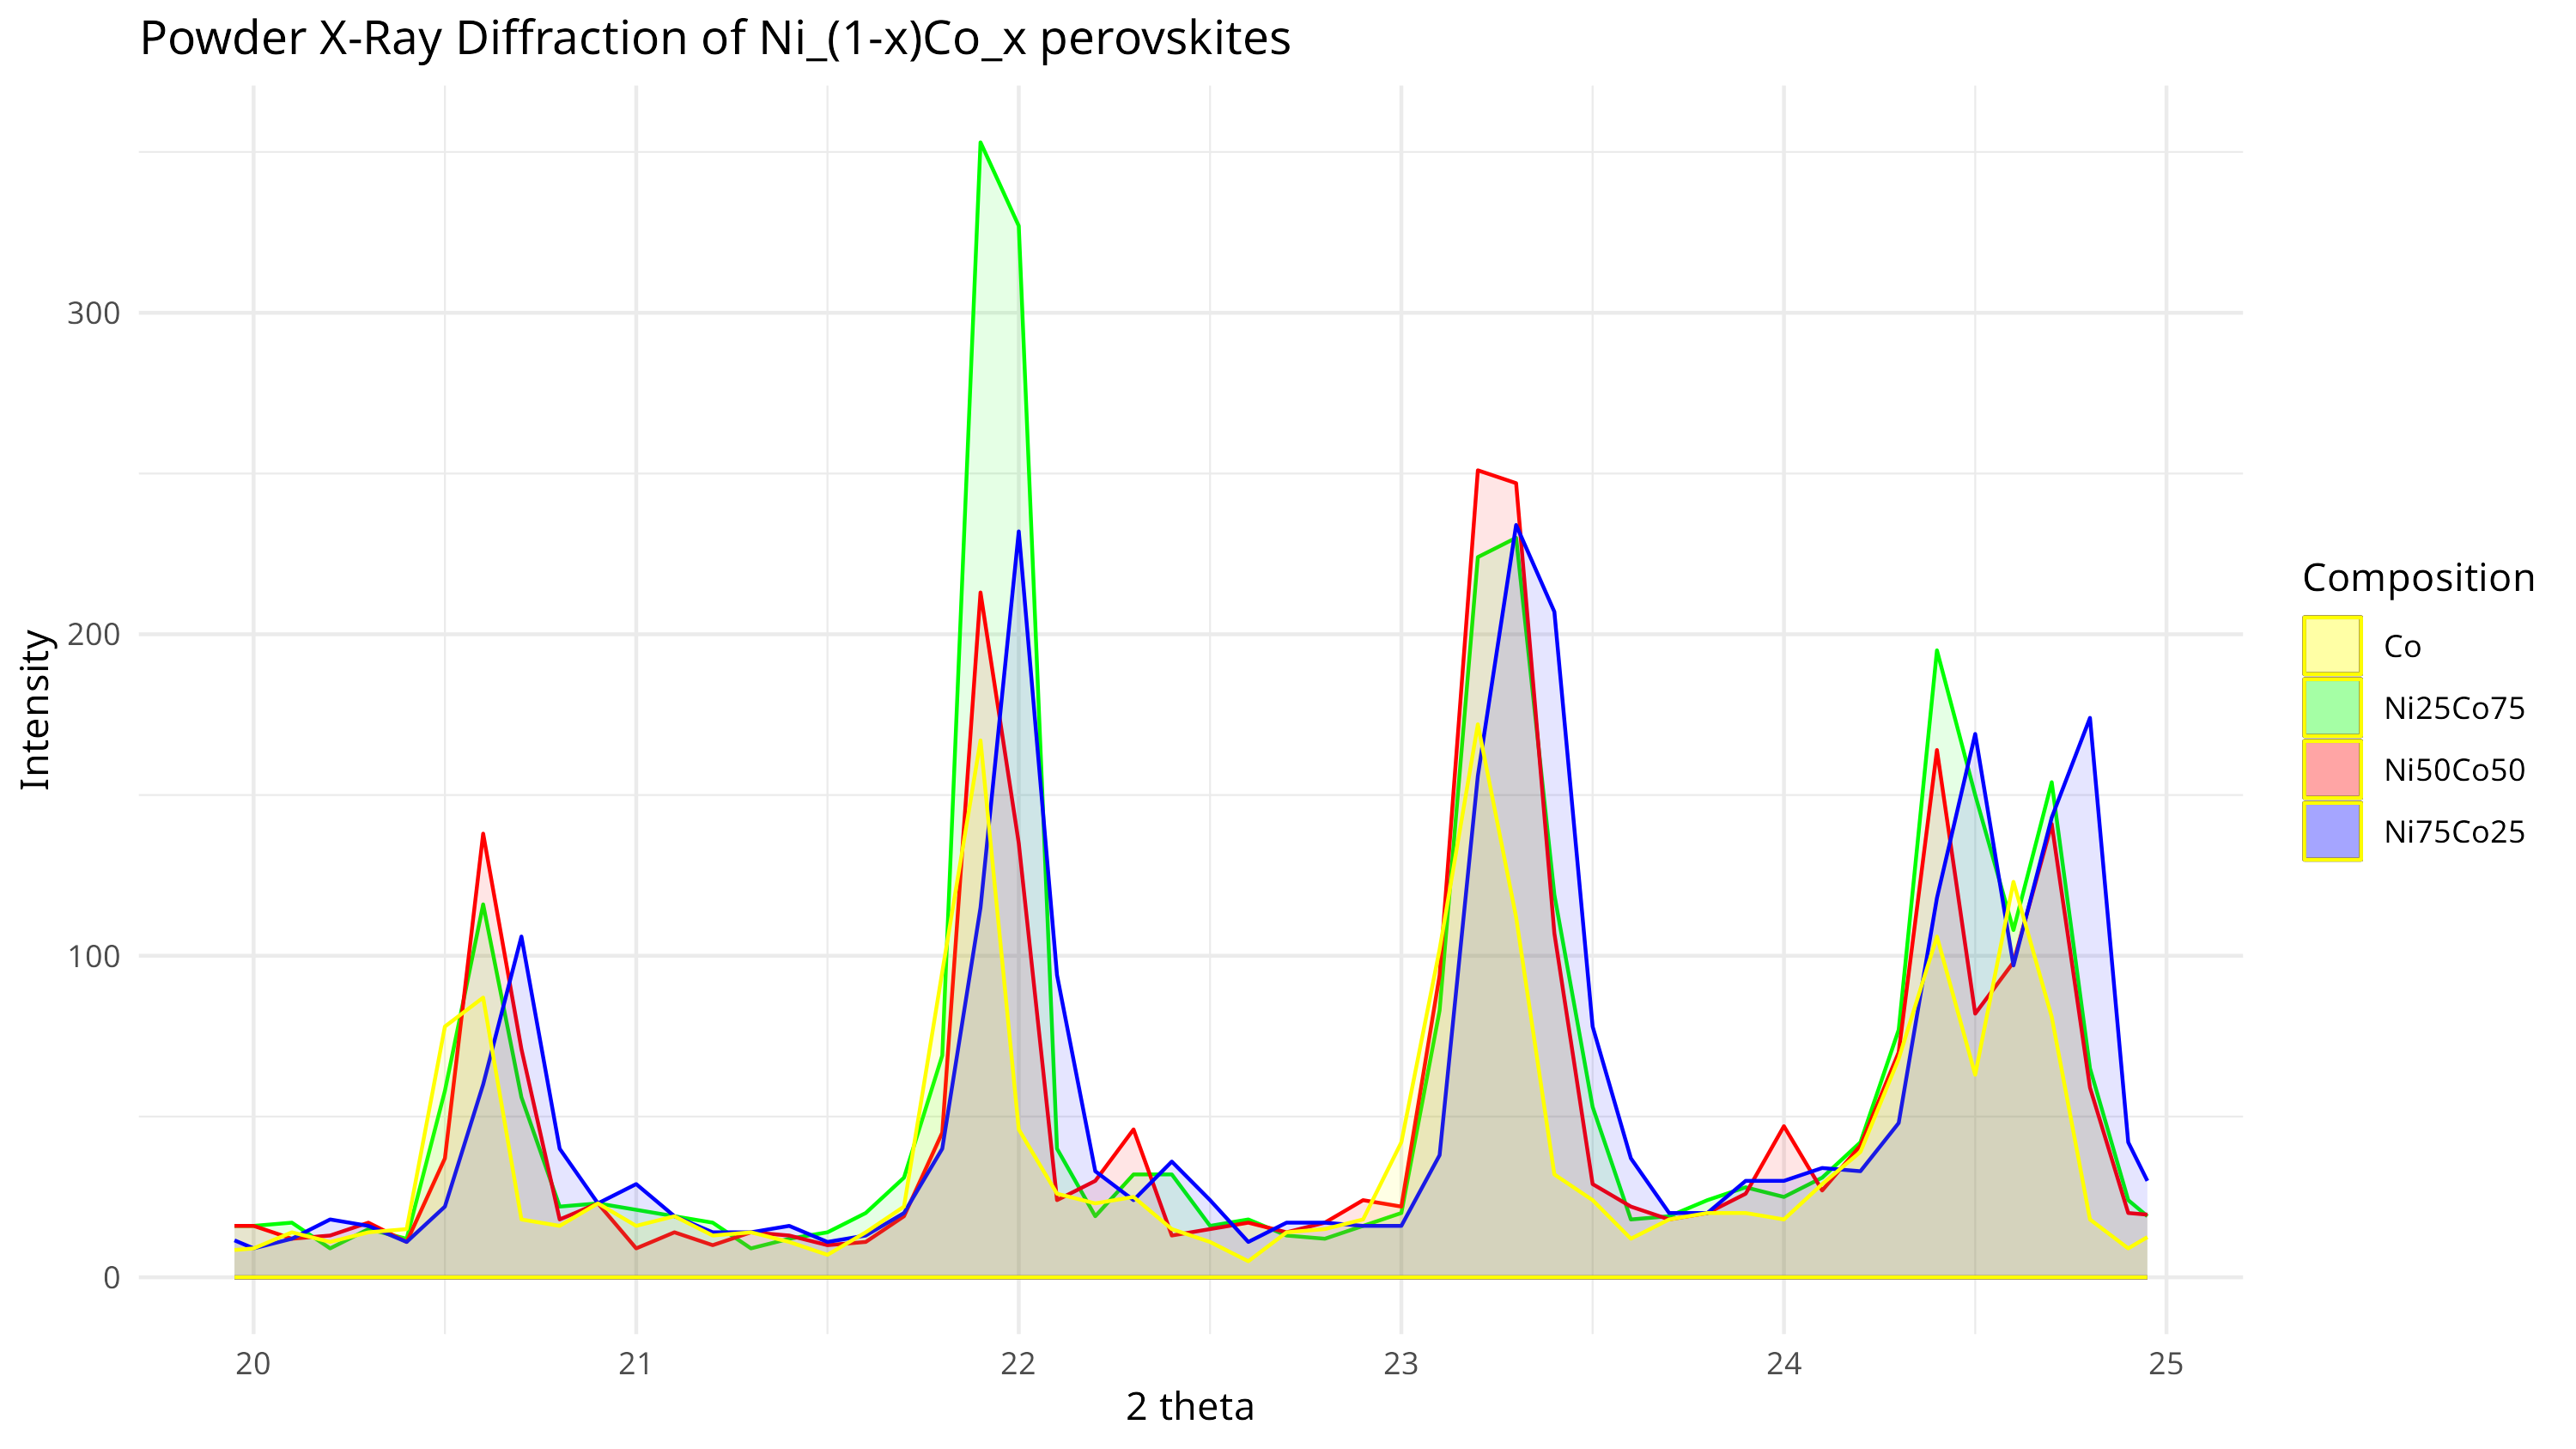
\includegraphics[width=1\textwidth]{../plot/graph_nb_zoom.png}
        \caption{Powder X-ray Diffraction of Ni\_(1-x)Co\_x perovskites}
        \label{fig:xrd}
    \end{figure}
\end{frame}

\begin{frame}[fragile]{Exploratory Data Analysis}
    \begin{itemize}
        \item Visualizations and summary statistics.
        \item Identification of patterns and trends.
    \end{itemize}

    \begin{lstlisting}[language=R, basicstyle=\tiny\ttfamily]
      #Threshold value
        +
      geom_hline(
        yintercept = threshold,
        linetype = "dashed", color = "black"
      )
    \end{lstlisting}
\end{frame}

\begin{frame}{Visualization of the Data}
    \begin{figure}
        \centering
        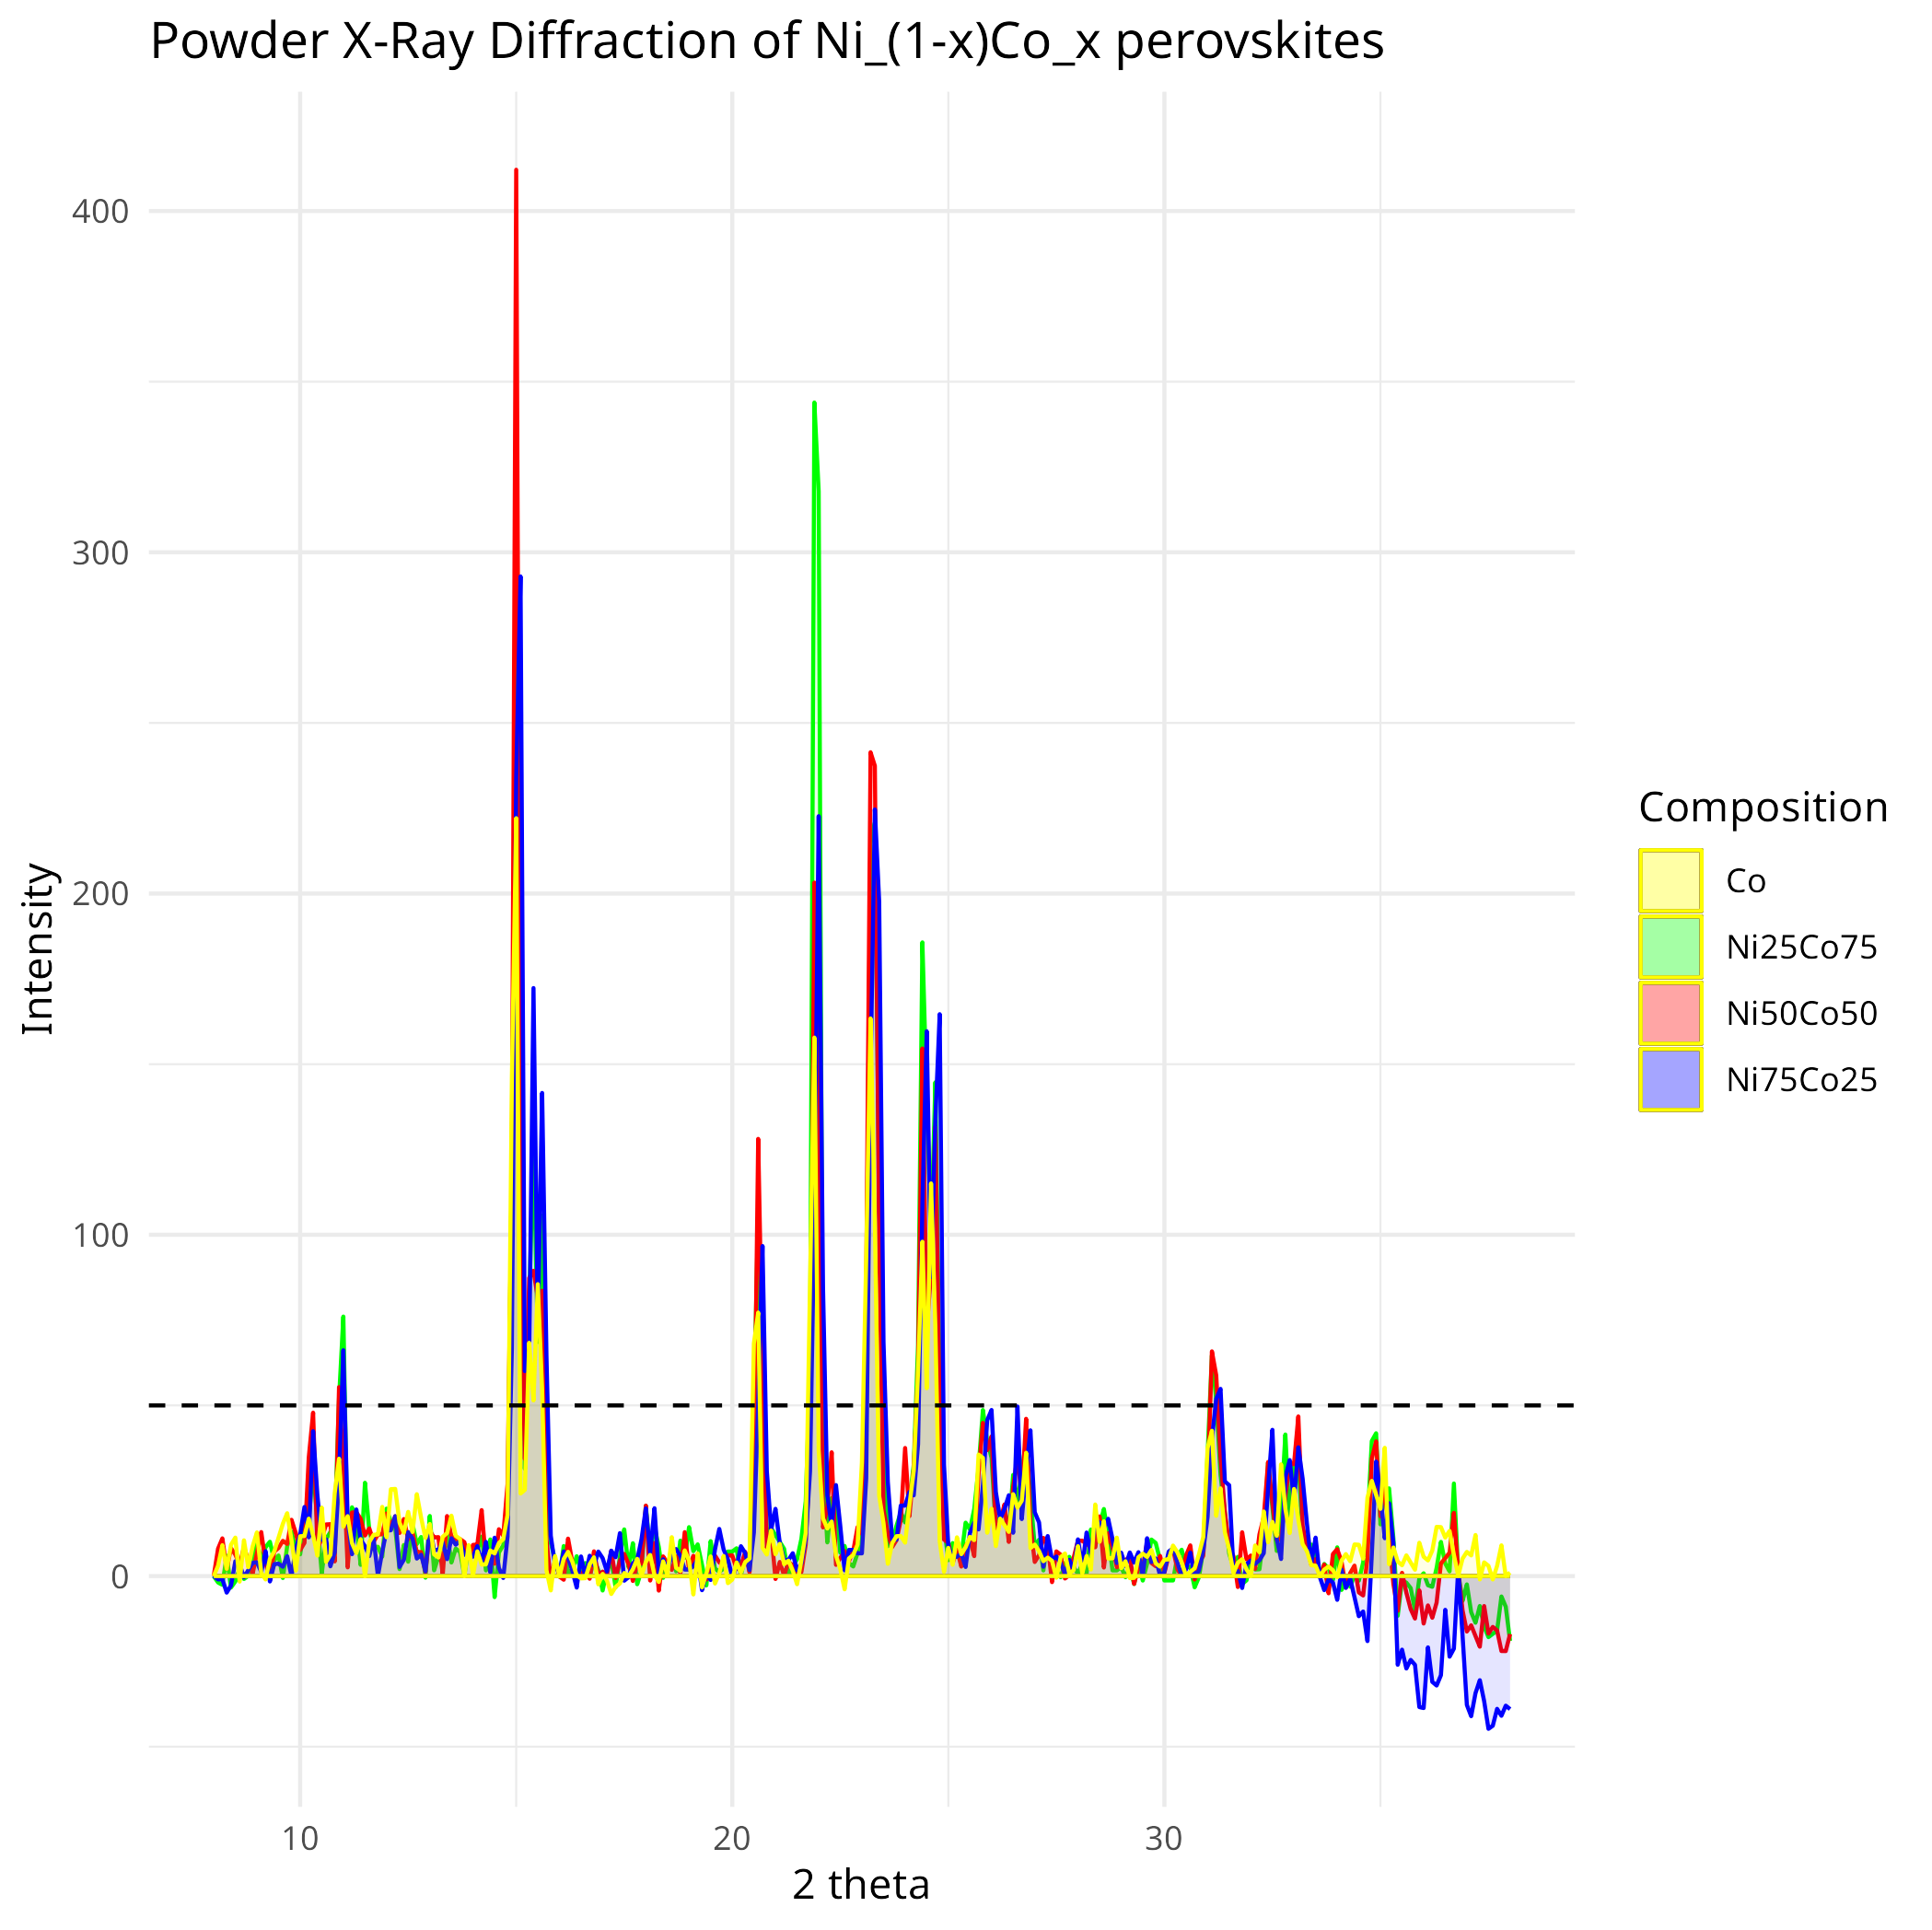
\includegraphics[width=1\textwidth]{../plot/graph.png}
        \caption{Powder X-ray Diffraction of Ni\_(1-x)Co\_x perovskites without background and with threshold value}
        \label{fig:xrd}
    \end{figure}
\end{frame}




\begin{frame}[fragile]{Peak Identification}
    \begin{itemize}
        \item Overview of the importance of identifying peaks in X-ray diffraction data.
        \item Explanation of the methodology used for peak identification.
    \end{itemize}

    \begin{lstlisting}[language=R, basicstyle=\tiny\ttfamily]
    find_peaks <- function(data) {
      if (length(data) < 2) {
        return(NULL) # No peak in lists with 0 or 1 element
      }
      peaks <- rep(0, length(data))
      # Create a vector to store the value and index of the peaks
      for (i in 2:(length(data) - 1)) {
        if (data[i] > data[i - 1] && data[i] > data[i + 1]) { # Looking for a peak
          peaks[i] <- data[i]
        }
      }
      # Checking if the first and last value is a peak or not
      if (data[1] > data[2]) {
        peaks[1] <- data[1]
      }
      if (tail(data, 1) > tail(data, 2)[1]) {
        peaks[length(peaks)] <- data[length(data)]
      }
      return(peaks)
      }    \end{lstlisting}
\end{frame}

\begin{frame}{Peak Identification Results}
    \begin{figure}
        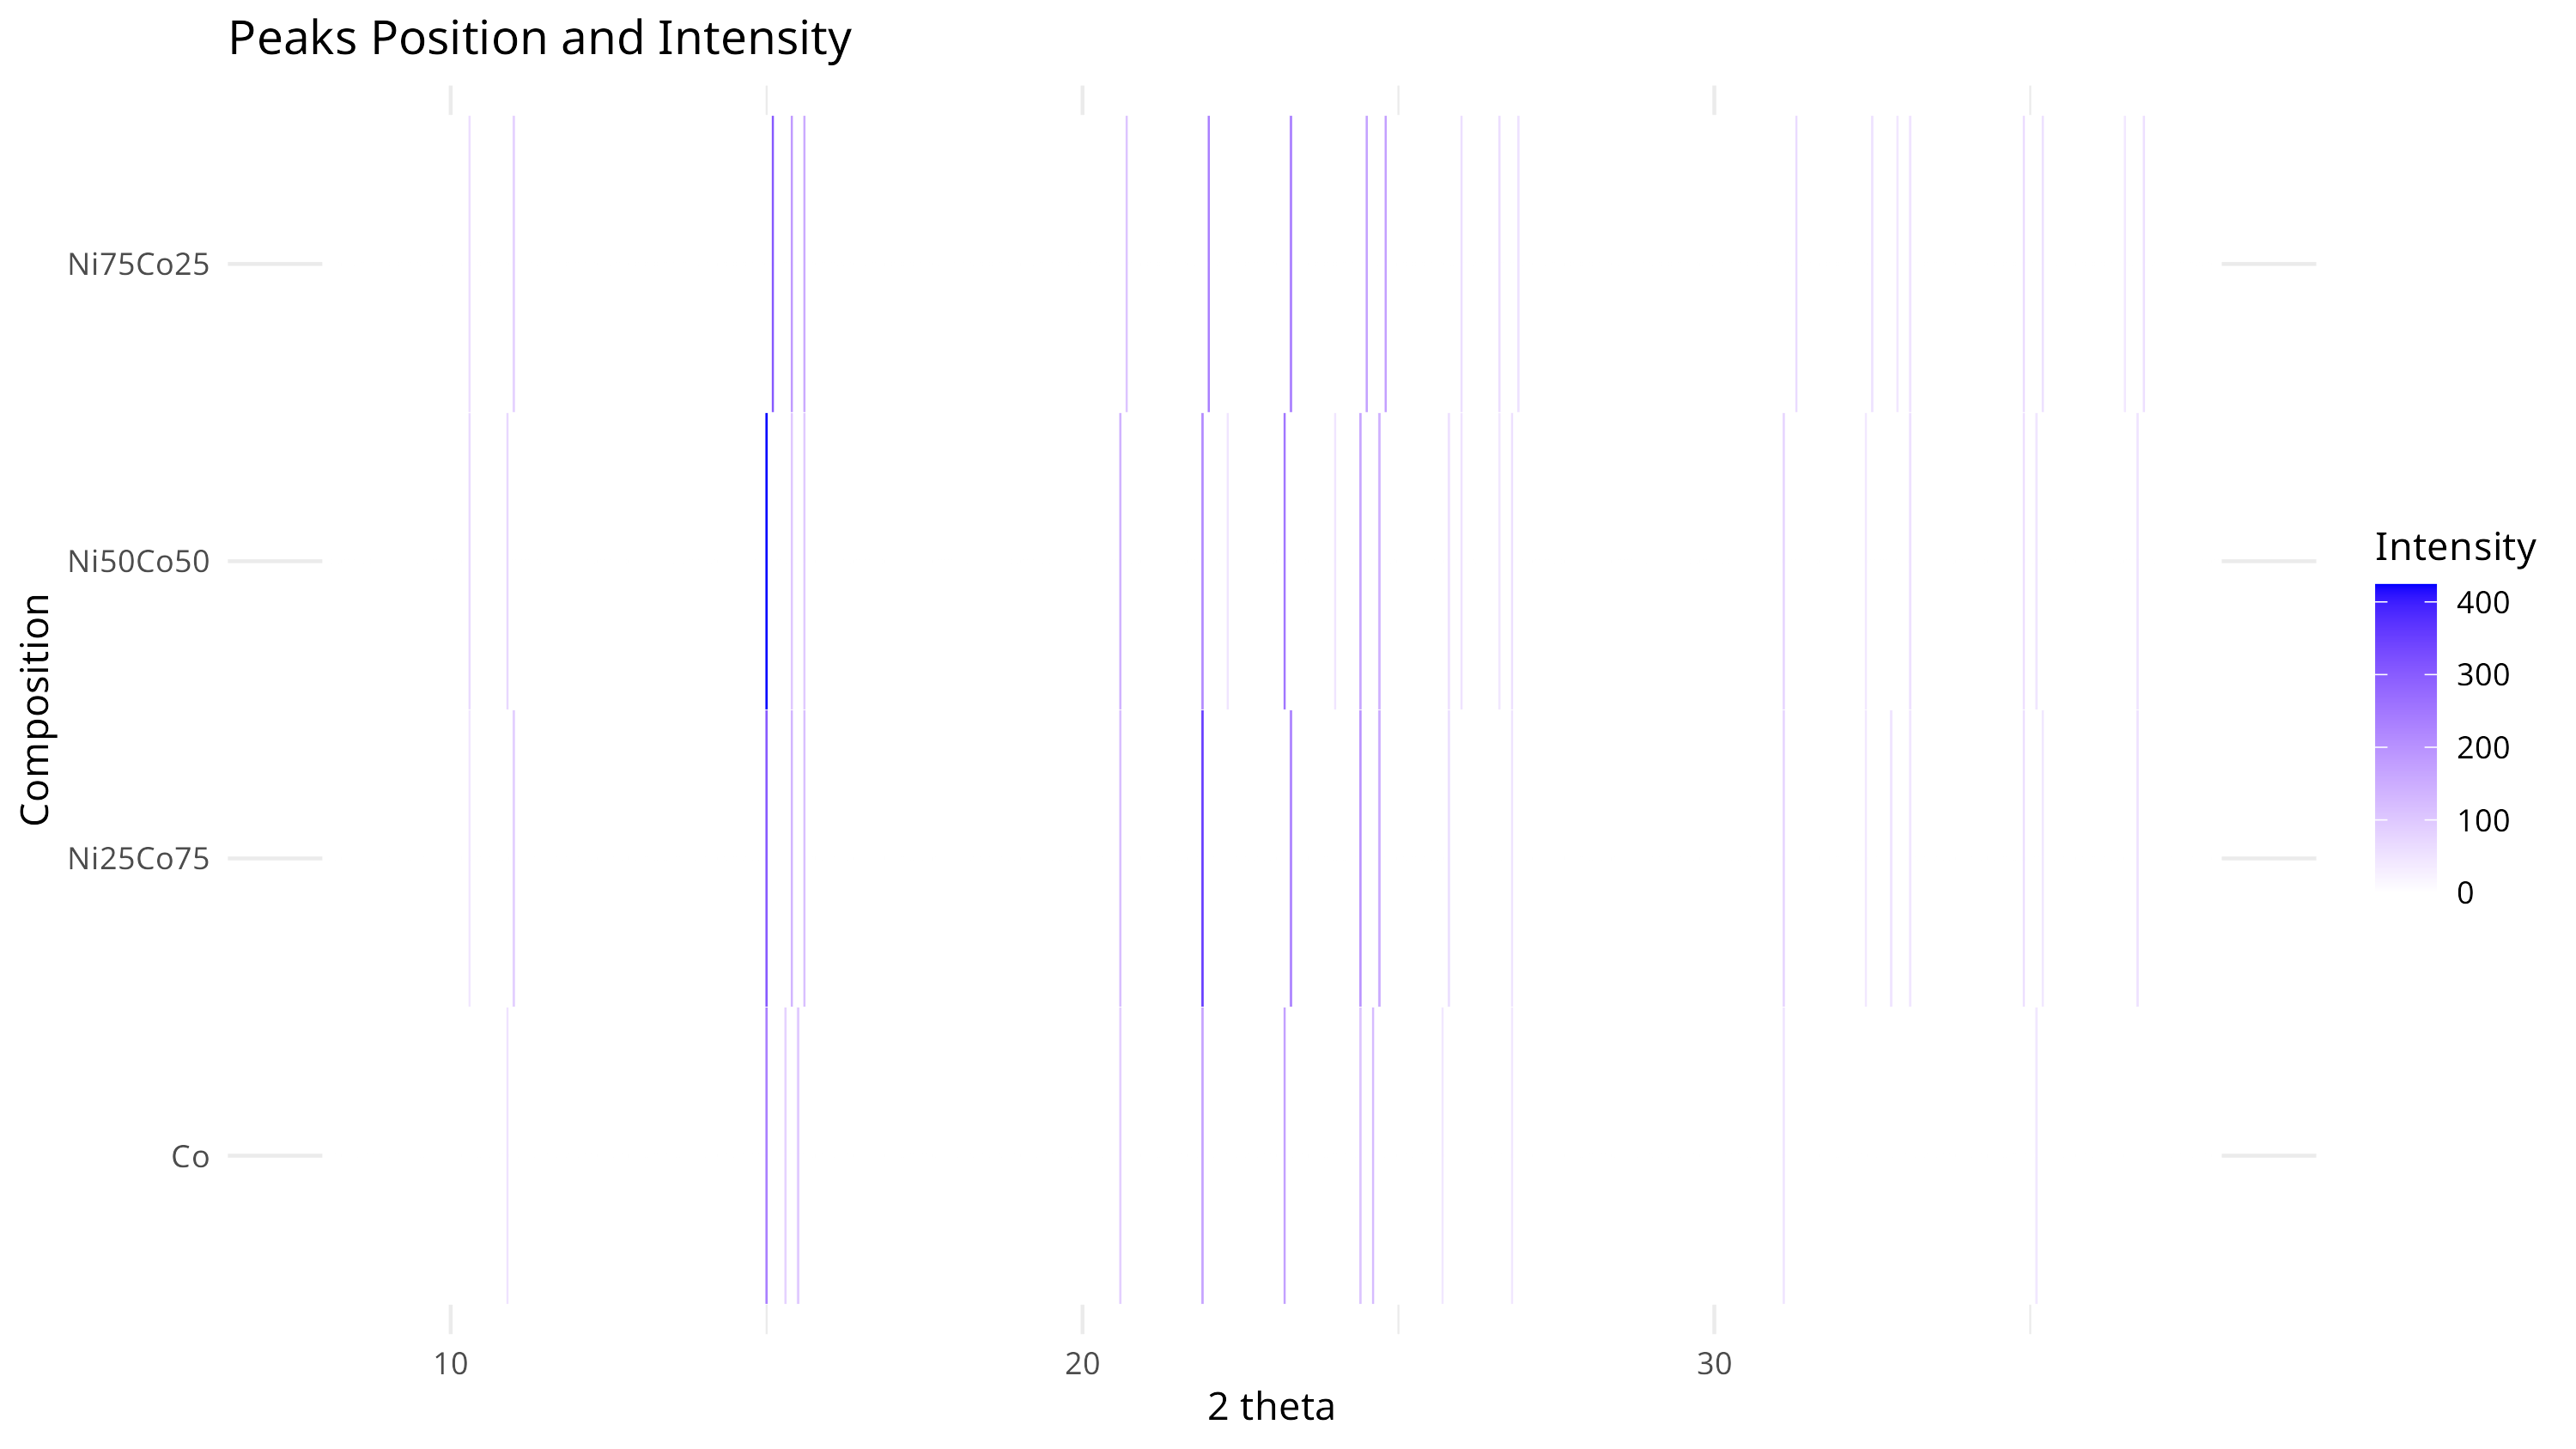
\includegraphics[width=1\textwidth]{../plot/peaks.png}
    \end{figure}
\end{frame}




\begin{frame}[fragile]{Clustering Process}
    \begin{itemize}
        \item Explanation of the clustering algorithm used.
        \item Description of the data preparation steps.
    \end{itemize}

    \begin{lstlisting}[language=R, basicstyle=\small\ttfamily]
    
# Specify the number of clusters (k)
      k <- 10

# Perform k-means clustering based only on 2_theta
      cluster_assignments <- kmeans(data_for_clustering,
        centers = k,
        nstart = 4
      )$cluster

    \end{lstlisting}
\end{frame}

\begin{frame}{Clustering Results}
    \begin{itemize}
        \item Overview of the clustering results.
        \item Interpretation of clusters and their characteristics.
    \end{itemize}

    \begin{figure}
        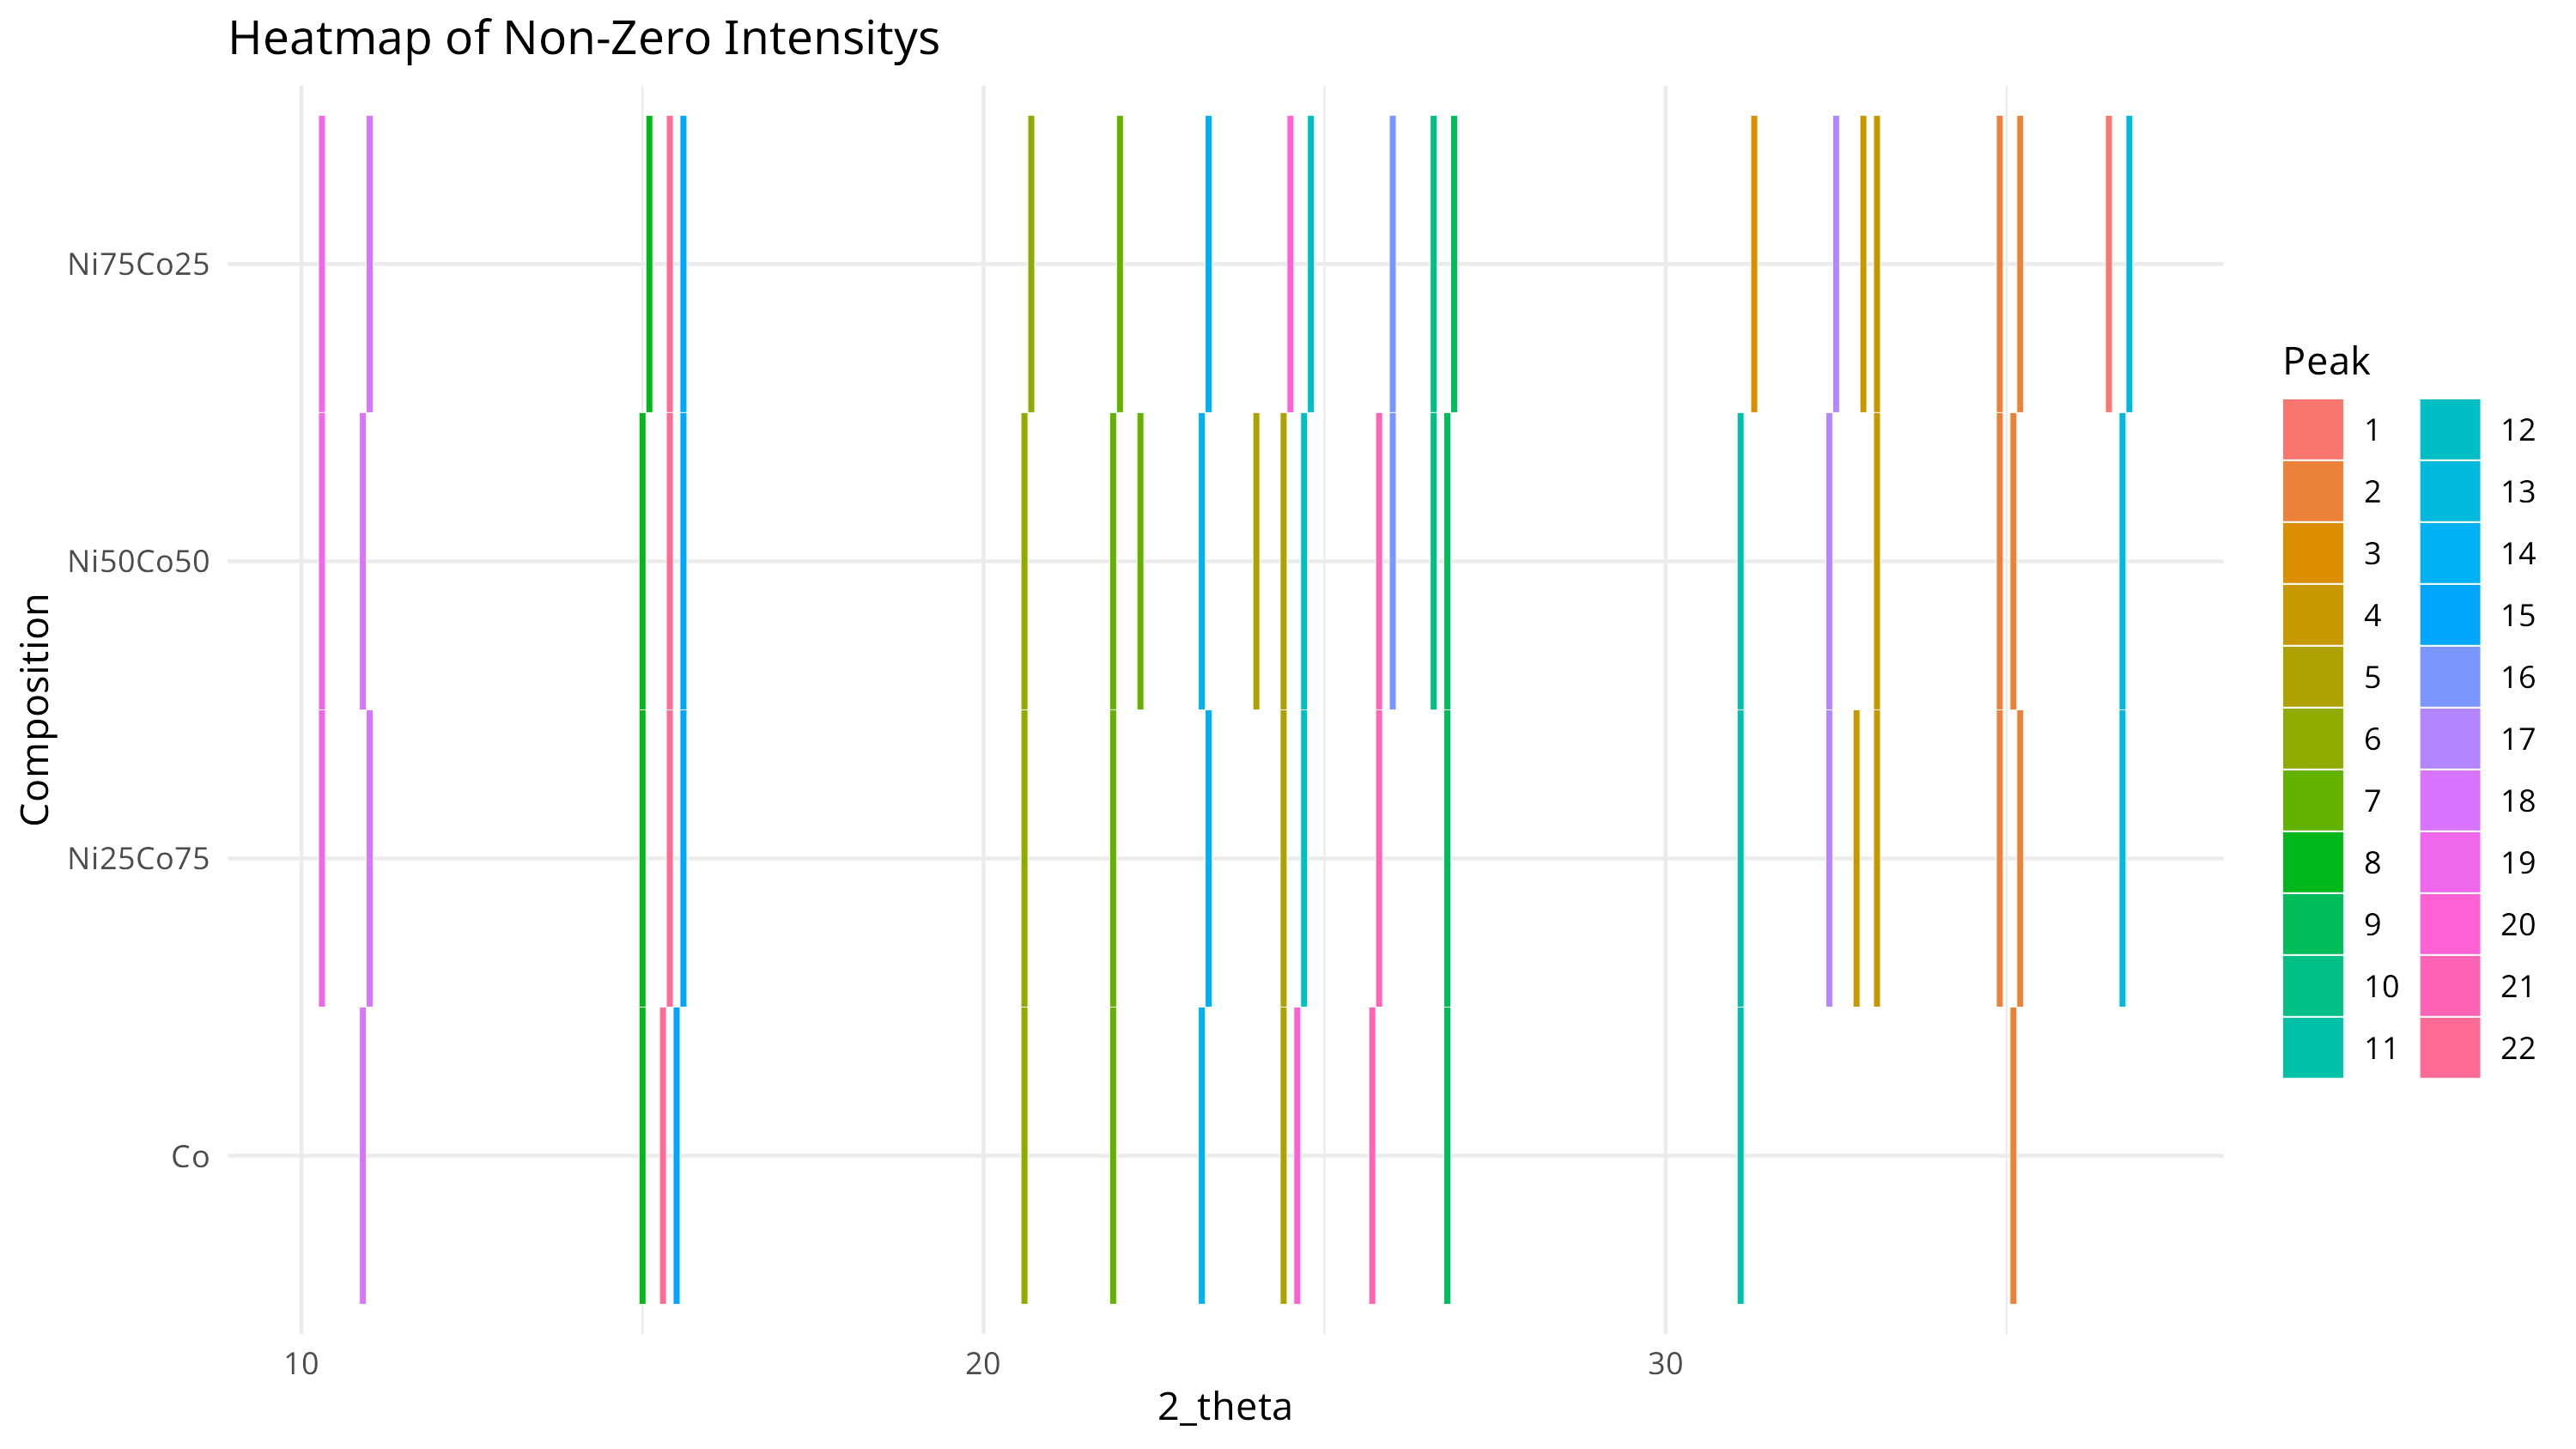
\includegraphics[width=0.5\textwidth]{../plot/peak_clusters.png}
        \caption{Clustering results visualized.}
    \end{figure}
\end{frame}

\begin{frame}{Clustering Results}
    \begin{itemize}
        \item Overview of the clustering results.
        \item Interpretation of clusters and their characteristics.
    \end{itemize}

    \begin{figure}
        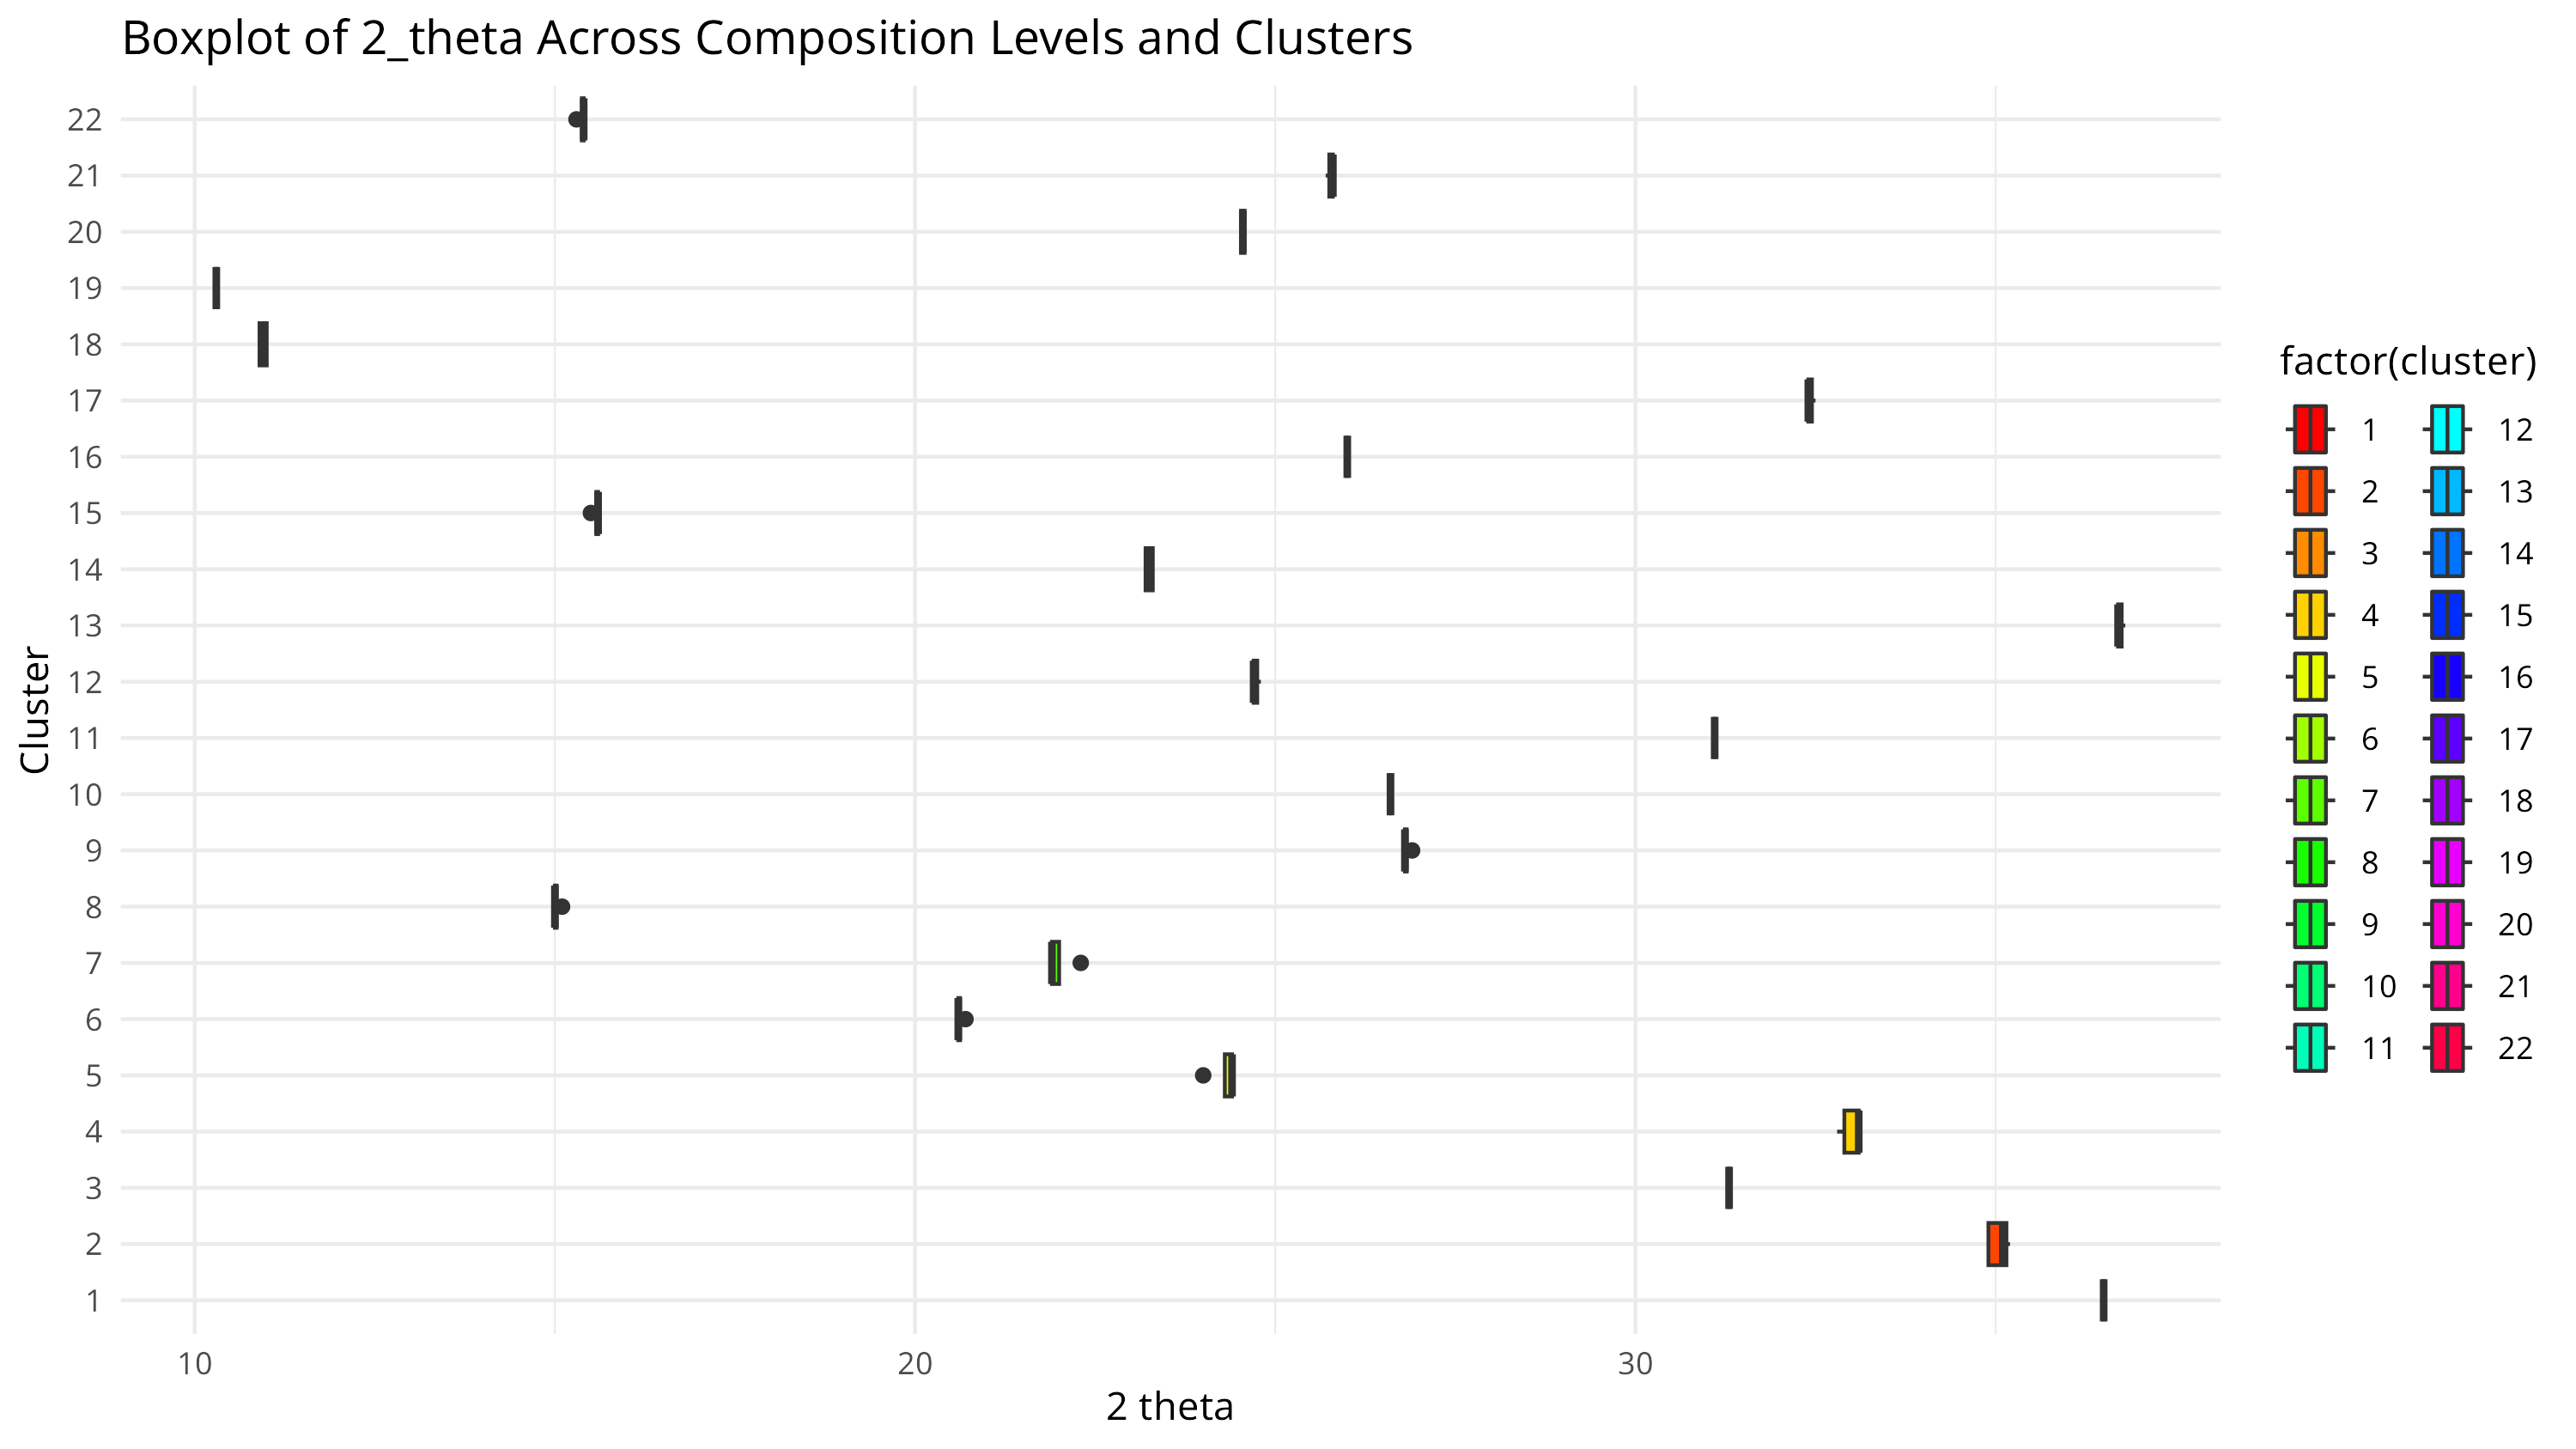
\includegraphics[width=0.85\textwidth]{../plot/theta.png}
        \caption{Clustering results visualized.}
    \end{figure}
\end{frame}

\begin{frame}[fragile]{ANOVA Results}
  \begin{lstlisting}[language=R, basicstyle=\small\ttfamily]
  # Perform ANOVA
  anova_result_composition <- aov(`2_theta` ~ Composition * cluster, data = non_zero_data_long)
  
  # Print ANOVA summary
  summary(anova_result_composition)
  \end{lstlisting}
\end{frame}


\begin{frame}{ANOVA Results}
  \begin{table}[]
    \centering
    \begin{tabular}{lcccccc}
      \hline
      \textbf{Factor} & \textbf{Df} & \textbf{Sum Sq} & \textbf{Mean Sq} & \textbf{F Intensity} & \textbf{Pr(>F)} \\
      \hline
      Composition & 3 & 0.5 & 0.15 & 5.137 & 0.0286* \\
      Cluster & 9 & 1103.8 & 122.65 & 4175.310 & $1.03 \times 10^{-13}$*** \\
      Composition:Cluster & 17 & 0.0 & 0.00 & 0.066 & 1.0000 \\
      Residuals & 8 & 0.2 & 0.03 & & \\
      \hline
    \end{tabular}
  \end{table}
  Signif. codes: 0 ‘***’ 0.001 ‘**’ 0.01 ‘*’ 0.05 ‘.’ 0.1 ‘ ’ 1
\end{frame}

\begin{frame}{Analysis of ANOVA Results}
  \begin{itemize}
    \item The Composition factor shows a significant effect on the response variable (p-value = 0.0286).
    \item The Cluster factor has a highly significant impact on the response variable (p-value = $1.03 \times 10^{-13}$).
    \item The interaction between Composition and Cluster is not significant (p-value = 1.0000).
    \item Residuals indicate the unexplained variance in the model.
  \end{itemize}
\end{frame}


\begin{frame}{Peak Intensity}
    \begin{itemize}
        \item Powder X-ray Diffraction (PXRD) data often contains peaks that correspond to specific crystallographic planes.
        \item Peak intensity is a crucial parameter in PXRD analysis, reflecting the abundance or concentration of particular crystallographic phases.
    \end{itemize}

    \begin{figure}
        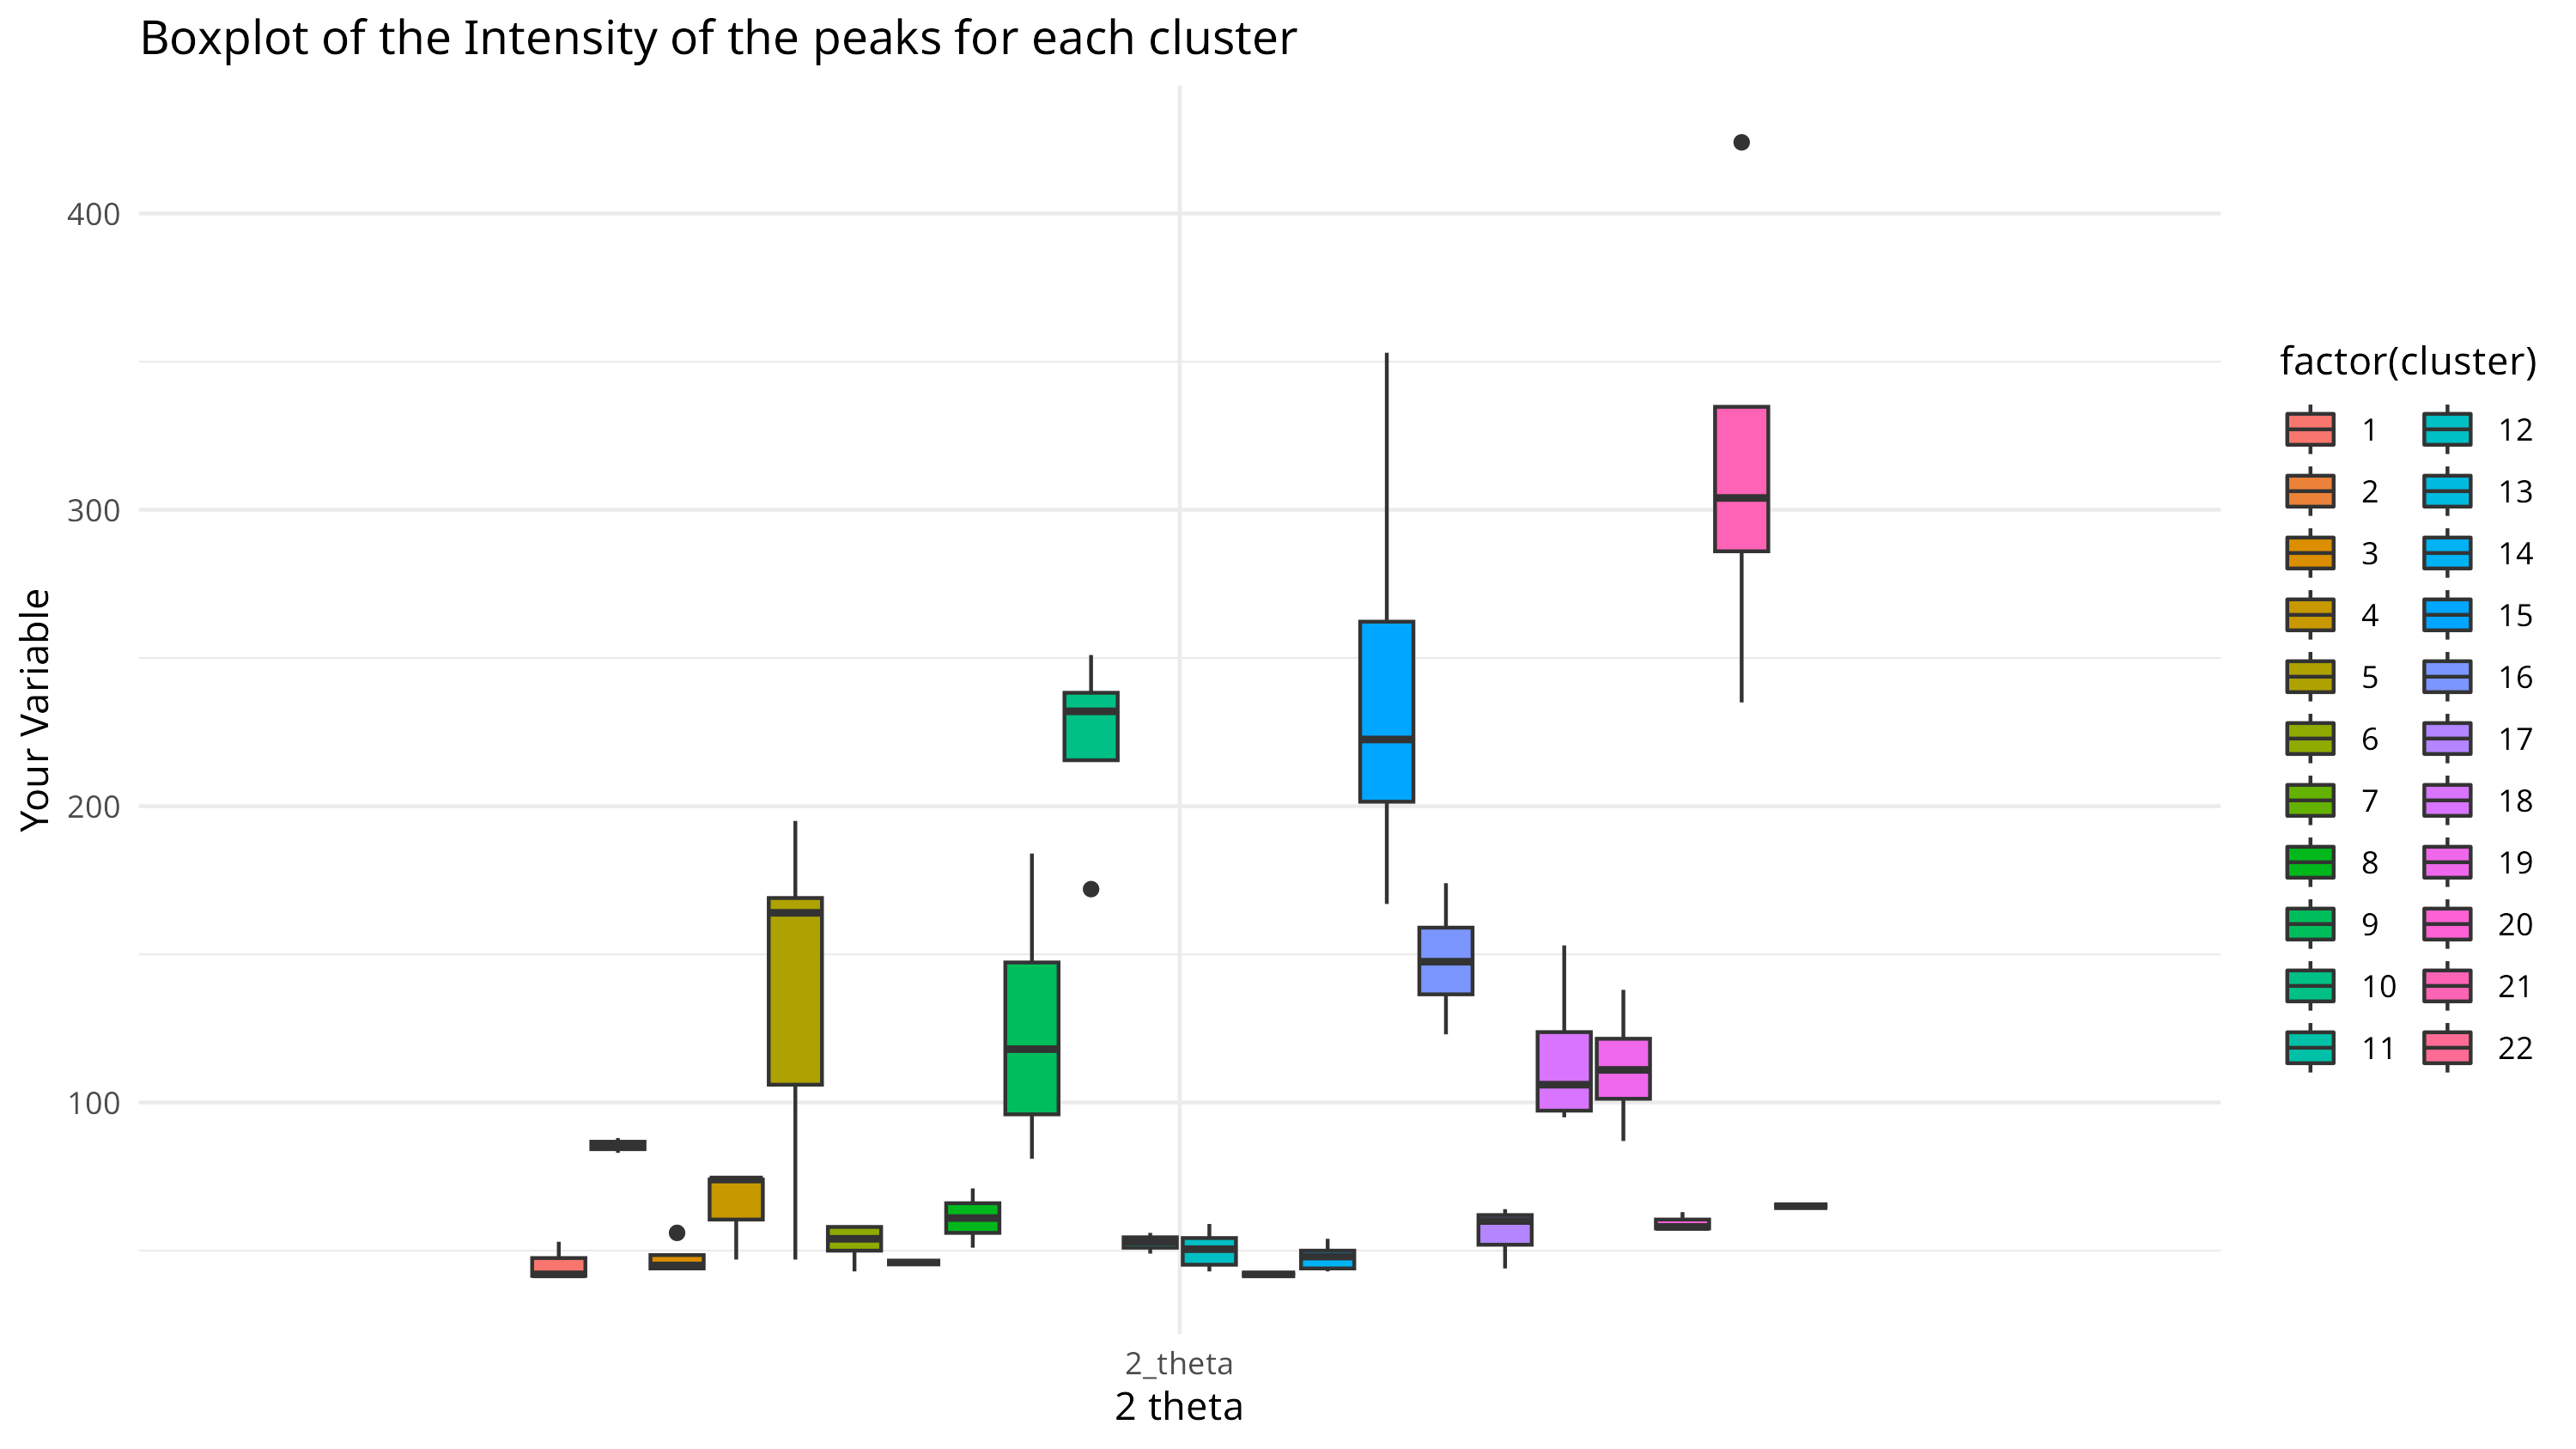
\includegraphics[width=0.7\textwidth]{../plot/intensity.png}
        \caption{Example of Powder X-ray Diffraction Peaks and Intensity.}
    \end{figure}

    \begin{itemize}
        \item Understanding peak intensity variations provides insights into material composition and structural characteristics.
        \item Our analysis focuses on identifying, characterizing, and comparing peak intensities in the given dataset.
    \end{itemize}
\end{frame}


\begin{frame}[fragile]{ANOVA Results}
    \begin{itemize}
        \item Analysis of Variance (ANOVA) was performed to assess the impact of 'Composition' and 'cluster' on the 'Intensity' variable.
        \item Statistical significance was evaluated based on p-values.
    \end{itemize}

    \begin{lstlisting}[language=R, basicstyle=\tiny\ttfamily]
      > anova_result <- aov(Intensity ~ Composition * cluster, data = non_zero_data_long)


      > summary(anova_result)
                        Df Sum Sq Mean Sq F value   Pr(>F)    
      Composition          3   9496    3165   14.80 0.012440 *  
      cluster            9 220856   24540  114.78 0.000182 ***
      Composition:cluster 21  31651    1507    7.05 0.035380 *  
      Residuals          4    855     214                     
      ---
      Signif. codes:  0 ‘***’ 0.001 ‘**’ 0.01 ‘*’ 0.05 ‘.’ 0.1 ‘ ’ 1   
\end{lstlisting}

    \begin{itemize}
        \item \textbf{Composition:} The p-value (0.012440) indicates a significant difference in means across 'Composition' levels.
        \item \textbf{Cluster:} A very low p-value (0.000182) suggests significant differences in means across clusters.
        \item \textbf{Interaction:} The interaction between 'Composition' and 'cluster' is significant (p-value = 0.035380).
    \end{itemize}
\end{frame}



\begin{frame}{Results and Discussion}
    \begin{itemize}
        \item Interpretation of ANOVA results.
        \item Comparison of clusters: Assessing the significance of peak position variations.
        \item Implications of the findings: Understanding how composition affects peak positions.
    \end{itemize}
\end{frame}



\begin{frame}{Conclusion}
  \begin{columns}
    \begin{column}{0.5\textwidth}
      \centering
      \textbf{\textcolor{blue}{Summary of key findings.}}
      \begin{itemize}
        \item Peak position,
        \item Intensity.
      \end{itemize}
    \end{column}
    
    \begin{column}{0.5\textwidth}
      \centering
      \textbf{\textcolor{red}{Limitations and areas for future research.}}
      \begin{itemize}
        \item \textbf{Ni} composition for further analysis,
        \item Improve the peak finding algorithm,
        \item Random variability in the clustering process.
      \end{itemize}
    \end{column}
  \end{columns}
\end{frame}



\begin{frame}{Questions \& Discussion}
    \centering
    \Huge Any Questions?
\end{frame}

\end{document}

